\section{Scale-Free Networks: Variations on the Theme}

As we have seen, the standard Barabási-Albert (B-A) model elegantly generates a scale-free topology, but it suffers from a major mathematical constraint: it produces a fixed, unmodifiable scaling exponent (\( \alpha = 3 \)). In reality, empirical networks exhibit a wide range of exponents (typically between 2 and 3) and display complex dynamics that the pure B-A model cannot capture.

To incorporate more general features and achieve more realistic macroscopic behavior, various modifications to the basic B-A model have been proposed. The four main variations are:
\begin{enumerate}
    \item \textbf{Attractiveness}
    \item \textbf{Fitness}
    \item \textbf{Node aging}
    \item \textbf{Generalized preferential attachment}
\end{enumerate}

\subsection{I Variation: Initial Attractiveness}

\subsubsection{Modifying the Preferential Attachment Rule}

The first variation introduces the concept of \textbf{Initial Attractiveness}. Let us consider a \textbf{directed network} model where, at each time step, \( m \) new connections are added to the network.
\textit{Note: Unlike the strict B-A model, this general framework does not mathematically require that all \( m \) new connections must originate strictly from the newly added node.}

In the pure B-A model, a node with zero links has a zero probability of acquiring new links. To overcome this "cold start" problem and model systems more realistically, we modify the preferential attachment rule. The probability \( p_{IN}(t) \) of a node receiving an \textit{incoming} link is no longer strictly proportional only to its current incoming connectivity \( K_{IN}(t) \). Instead, we add a constant baseline value \( A \), which represents the inherent \textbf{attractiveness} of the node:
\[
    p_{IN}(t) \propto K_{IN}(t) + A \quad \text{with} \quad A \geq 0
\]
Because \( A \geq 0 \), even a newly born node with \( K_{IN} = 0 \) possesses a non-zero probability of attracting links from the very beginning.

\subsubsection{Tuning the Scaling Exponent}

The profound mathematical consequence of adding this simple constant \( A \) is that it alters the asymptotic behavior of the network. Analytical demonstrations show that as the network grows, the distribution of incoming connectivity tends toward a power-law:
\[
    p_{IN}(K) \propto K_{IN}^{-\gamma}
\]
However, the scaling exponent \( \gamma \) is no longer locked at 3. It is now a function of the attractiveness \( A \) and the number of links added per step \( m \):
\[
    \gamma = 2 + \frac{A}{m}
\]
Since \( A \geq 0 \) and \( m > 0 \), the term \( A/m \) is always positive. This means that by simply varying the initial attractiveness parameter \( A \), we can theoretically generate scale-free networks with \textbf{any exponent greater than 2} (\( \gamma \geq 2 \)). This flexibility allows the model to perfectly fit the degree distributions observed in real-world empirical data.

\subsubsection{Node-Specific Attractiveness and the Mean Field}
While the equation above uses a single constant \( A \) for the entire network, assuming that an initial attractiveness value is exactly equal for \textit{all} nodes does not seem very biologically or technologically realistic.

To make the model physically plausible, we can interpret \( A \) as an \textbf{average value}. We can conceptualize more advanced models where attractiveness is \textbf{node-specific} (each node \( i \) is born with its own unique \( A_i \)). As long as the variance of these individual attractiveness values remains finite, the overall system will still produce the exact same \textbf{"mean field"} macroscopic behavior, correctly converging to the expected scale-free distribution.

\subsection{II Variation: Node Fitness}

\subsubsection{Overcoming the "Older Get Richer" Paradigm}

A major limitation of the standard Barabási-Albert (B-A) model is its strict reliance on the \textbf{"older get richer"} (or first-mover advantage) paradigm. Because node degree grows strictly as a function of time, the oldest nodes are mathematically guaranteed to become the largest hubs.

However, in real-world networks, a latecomer can still become a massive hub if it possesses intrinsically superior qualities (e.g., a highly innovative paper published recently might quickly surpass a mediocre paper published decades ago, or a new social media platform might rapidly drain users from an older one). To model this, we introduce the concept of a different growth speed for different nodes based on their inherent \textbf{fitness}.

\subsubsection{The Fitness Parameter (\( \eta \))}

We assign a specific fitness parameter \( \eta_i \) to each node \( i \). The preferential attachment rule is then modified so that the probability of acquiring a new link depends on both the node's current degree \( k_i(t) \) \textit{and} its fitness \( \eta_i \).

The modified link probability is:
\[
    p_i(t) = \frac{\eta_i \cdot k_i(t)}{\sum_j \eta_j \cdot k_j(t)}
\]
In this competitive model (often called the Bianconi-Barabási model), a younger node with a very high fitness \( \eta \) can acquire links at a much faster rate than an older node with a low fitness, eventually overtaking it in degree.

\subsubsection{Impact on the Degree Distribution}

The resulting degree distribution \( p(k) \) of the network is no longer a simple, fixed power-law; it now heavily depends on the underlying \textbf{node fitness distribution} \( p(\eta) \).

Analytical solutions show that different fitness distributions yield entirely different network topologies:
\begin{itemize}
    \item \textbf{Uniform fitness distribution:} If \( p(\eta) \) is uniform, the degree distribution picks up a logarithmic correction and scales as:
          \[
              p(k) \approx \frac{k^{-2.25}}{\log(k)}
          \]
    \item \textbf{Exponential fitness distribution:} If \( p(\eta) \) is exponential, the network loses its pure power-law tail entirely. Instead, the degree distribution becomes a \textbf{stretched exponential}:
          \[
              p(k) \propto e^{-t^b} \quad \text{with} \quad 0 < b < 1
          \]
          \textit{(Note: While the slide uses \( t \) in the exponent, in standard network literature this stretched exponential is typically expressed in terms of the degree as \( e^{-c \cdot k^b} \), indicating a decay that is faster than a power-law but slower than a pure exponential).}
\end{itemize}

\subsubsection{Robustness of the B-A Model}

Introducing fitness makes a lot of sense in real situations (e.g., modeling consensus forming around new opinions, or the spread of innovative scientific papers).

However, as demonstrated by the equations above, introducing fitness \textbf{destroys the strict scale-free property} of the network. This reveals a fundamental theoretical insight: the pure B-A model is \textbf{not very robust to perturbations}. Minor, highly realistic tweaks to its generative rules completely alter its asymptotic macroscopic behavior.

\begin{example}[Citation Networks]
    These fitness dynamics are particularly relevant when studying \textbf{citation networks}, which represent excellent candidates for practical network analysis projects.

    For example, utilizing a full database dump of PubMed (accessible in real-time via PubMed APIs), we can construct a network where:
    \begin{itemize}
        \item \textbf{Node} = Scientific paper
        \item \textbf{Link} = Citation (directed link from a newer paper to an older one)
    \end{itemize}

    In such a project, one can characterize network features as a function of specific node attributes. For instance, analyzing the citation growth speed (the effective "fitness") of a paper as a function of its characteristics, its authors, the publishing journal, or its specific research topic.
\end{example}

\subsection{III Variation: Node Ageing}

\subsubsection{The Concept of Ageing in Networks}

In the standard Barabási-Albert model, a node continues to accumulate links indefinitely as long as the network grows. However, in many real-world systems, this is highly unrealistic. For example, in a citation network, older papers typically stop receiving new citations after a certain period as the scientific focus shifts to newer discoveries.

To simulate this "aging" of nodes, researchers have considered different rules. We will explore two primary mechanisms: one that is analytically tractable (leading to sudden inactivation) and another that models a gradual decay of attractiveness.

\subsubsection{Ageing Rule 1: Sudden Inactivation (Exponential Cutoff)}

The first mechanism assumes that each node has a \textbf{constant chance of becoming "inactive"} at any given moment. Once a node becomes inactive, it "dies" from a network growth perspective and can no longer receive any new incoming links.

Because the probability of deactivation is constant at each step, the "active life" \( T \) of each node follows a discrete \textbf{geometric distribution}. If we divide time into small intervals \( \delta \) and assign a probability \( P \) of deactivation in each interval, the probability that a node survives longer than \( n \) intervals is:
\[
    p(T > n\delta) = (1 - P)^n
\]
The expected average active lifetime is therefore:
\[
    \langle T \rangle = \frac{\delta}{P}
\]
If we move to the continuous limit (where the time intervals become infinitely small, \( n \to \infty \) and \( \delta \to 0 \)), and we define a characteristic time constant \( \alpha = \delta / P \), the geometric distribution cleanly converges to an \textbf{exponential law}:
\[
    \lim_{\substack{n \to \infty \\ \delta \to 0 \\ \delta/P = \alpha}} p(T > t = n\delta) = \left(1 - \frac{\delta}{\alpha}\right)^{\frac{t}{\delta}} = e^{-\frac{t}{\alpha}}
\]

\textbf{Topological Consequence:}
This aging mechanism fundamentally alters the degree distribution. By giving nodes a finite expected lifespan, we prevent the oldest nodes from growing infinitely large. This introduces an \textbf{exponential cutoff} to the power-law distribution. For sufficiently large values of \( k \), the exponential term dominates and "dumps" the scale-free effect, resulting in a \textbf{Gamma-like distribution}:
\[
    p(k) \propto k^{-\alpha} e^{-\beta k}
\]

\begin{figure}[H]
    \begin{minipage}{0.35\textwidth}
        \caption{Schematic log-log plot of the degree distribution \( P(k) \) vs. \( k \) for a network with node aging. The plot should show three curves: "No aging" (a straight line representing the pure power-law), "Slow aging" (a curve that follows the power-law initially but bends downward at the tail), and "Fast aging" (a curve that cuts off and drops down much earlier due to rapid node inactivation).}
    \end{minipage}
    \hfill
    \begin{minipage}{0.6\textwidth}
        \centering
        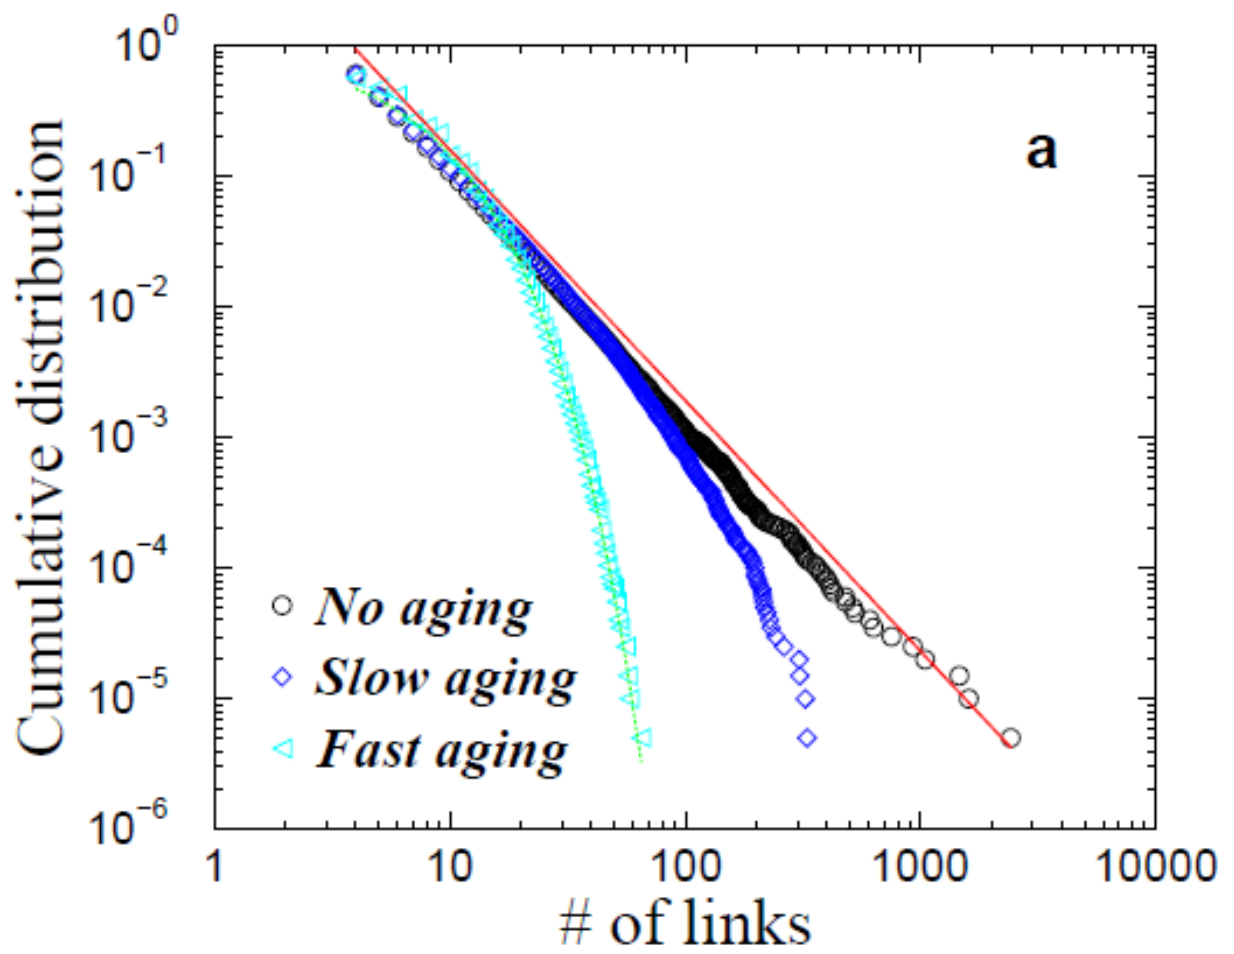
\includegraphics[width=0.8\textwidth]{img/aging_cutoff.png}
    \end{minipage}

\end{figure}

\subsubsection{Ageing Rule 2: Gradual Decay of Preferential Attachment}

The second mechanism models aging not as a sudden death, but as a gradual loss of relevance. The preferential attachment rule is modified such that a node's ability to attract new links decays over time \( t \) following a power-law governed by an aging parameter \( \beta \).

The modified probability of acquiring a link becomes:
\[
    p_i(t) \propto \frac{k_i(t)}{t^\beta}
\]
The resulting network topology is exquisitely sensitive to the chosen value of \( \beta \):
\begin{itemize}
    \item \textbf{Strong Ageing (\( \beta > 1 \)):} The attractiveness decays so quickly that the preferential attachment mechanism is effectively neutralized. The network \textbf{loses its scale-free behavior} entirely.
    \item \textbf{Moderate Ageing (\( 0 < \beta < 1 \)):} The network maintains a scale-free power-law distribution (\( p(k) \propto k^{-\gamma} \)), but the aging parameter increases the scaling exponent beyond the standard B-A limit. Specifically, the exponent falls into the range:
          \[
              3 < \gamma < \infty
          \]
\end{itemize}

\subsubsection{Summary: Ageing and Open Systems Dynamics}

Incorporating an aging mechanism—which is highly plausible in almost all social, biological, and technological networks—increases the "elasticity" of the generative model. Depending on the exact rules and parameters, aging can either:
\begin{enumerate}
    \item Introduce exponential cutoffs that destroy the pure scale-free distribution at the extreme tail.
    \item Provide a way to smoothly scale the exponent \( \gamma \) within a limited regime of parameters.
\end{enumerate}

Finally, when dealing with open systems, we can also consider models that incorporate explicit \textbf{node birth and death} rates. While many real systems simply grow over time, some maintain a constant number of active nodes by balancing birth and death.
This dynamic framework raises interesting questions for real-world modeling: \textit{What happens to the topology if the network undergoes a sudden "inflation period" characterized by drastically increased, exponential node growth?}

\subsection{IV Variation: Generalized Preferential Attachment}

The standard Barabási-Albert model relies on a strictly linear preferential attachment rule, where the probability of a node receiving a link is exactly proportional to its degree (\( p_i \propto k_i \)).

However, we can generalize this mechanism by assuming that the probability depends on a \textbf{nonlinear power} of the node's degree. We introduce an attachment exponent \( \alpha \), leading to the generalized probability:
\[
    p_i(t) = \frac{k_i(t)^\alpha}{\sum_j k_j(t)^\alpha}
\]
Depending on the value of this new parameter \( \alpha \), the network dynamics enter completely different macroscopic regimes.

\subsubsection{Sub-linear Regime: \( 0 < \alpha < 1 \)}

In this regime, the attachment is \textit{less than proportional}. The "rich get richer" mechanism is weakened, meaning hubs do not grow fast enough to sustain a pure power-law distribution.

Consequently, the scale-free nature is destroyed. The limit degree distribution becomes a \textbf{stretched exponential}:
\[
    p(k) \approx e^{-\mu \cdot k^{1-\alpha}} \quad \text{with} \quad 1 \leq \mu \leq 2
\]

\subsubsection{Super-linear Regime: \( \alpha > 1 \)}

If \( \alpha > 1 \), the attachment is \textit{more than proportional}. The "rich get richer" effect becomes overwhelmingly strong, leading to a "winner-takes-all" dynamic.

In statistical mechanics, this corresponds perfectly to \textbf{Bose-Einstein condensation}. In the thermodynamic limit (as the network grows infinitely large), a single "super-hub" node emerges and aggressively collects a finite, macroscopic portion of all the links in the entire system. Because this single node monopolizes the connections, very few links remain for the rest of the network.
Topologically, the network collapses and approximates a massive \textbf{star graph}.

\subsubsection{Asymptotic Linear Behavior}

We know that for exactly proportional attachment (\( \alpha = 1 \)), we recover the standard B-A distribution:
\[
    p(k) \propto k^{-3}
\]
However, we can obtain different scaling exponents by introducing an attachment rule that is non-linear for small degrees, but \textbf{becomes linearly proportional only in the limit of large degrees} (\( k \gg 1 \)).

Mathematically, we require that the attachment probability asymptotically approaches a linear function:
\[
    p_i(t) \xrightarrow{k \to \infty} a_\infty k
\]
An example of such a function is:
\[
    p_i(t) = \frac{k_i}{k_i + a} \cdot k_i
\]
For small values of \( k_i \), the function is non-linear. But for very large hubs (\( k_i \gg a \)), the fraction \( \frac{k_i}{k_i + a} \) tends to 1, and the probability scales strictly as \( k_i \).

\begin{figure}[H]
    \begin{minipage}{0.6\textwidth}
        \centering
        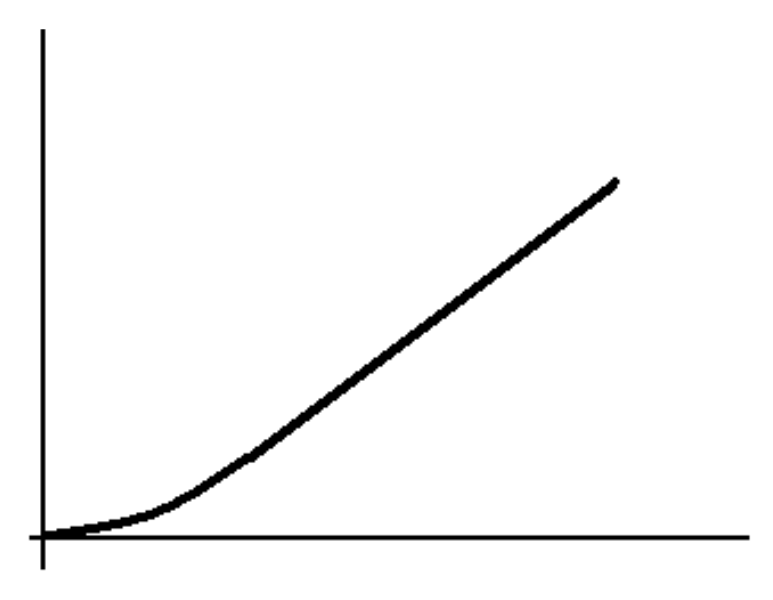
\includegraphics[width=0.8\textwidth]{img/generalized_pa.png}
    \end{minipage}
    \hfill
    \begin{minipage}{0.35\textwidth}
        \caption{Graph of the generalized preferential attachment function \( p_i(k) \) as a function of \( k \). The curve should start non-linearly near the origin (for small \( k \)) and asymptotically approach the straight diagonal line \( p_i(k) \approx a_\infty k \) for large \( k \).}
    \end{minipage}
\end{figure}

By carefully tuning these asymptotically linear rules, it is possible to mathematically generate scale-free networks capable of displaying \textbf{all possible exponents greater than 2}.

\subsubsection{Summary Note: Robustness of the B-A Model}

These four variations (Attractiveness, Fitness, Ageing, and Generalized PA) collectively highlight a fundamental conclusion regarding the Barabási-Albert model: \textbf{scale-free network generation purely via standard preferential attachment is not very robust.}

Even slight, highly realistic variations to the original B-A rules can radically modify the resulting topology—introducing exponential cutoffs, stretching the distributions, or condensing the network completely. Therefore, when modeling real complex systems, the specific underlying generative mechanisms must be carefully chosen to match empirical observations.

\subsection{Final Observations: Fat-Tails and the Non-Locality Problem}

To conclude the discussion on the Barabási-Albert model and scale-free networks, we must address some fundamental critical observations regarding their applicability to real-world systems.

\subsubsection{Are there any real scale-free networks?}

A rigorous mathematical definition of a scale-free network implies a pure power-law degree distribution that extends indefinitely. However, in any physical, biological, or technological system, \textbf{the infinite limit is never reached}. Finite size constraints inherently truncate the degree distribution.

Because of this, many real-world networks that are colloquially called "scale-free" are actually more accurately described as simply having \textbf{fat-tailed distributions} (or heavy-tailed). While they exhibit highly heterogeneous connectivity and the presence of hubs, their exact statistical distribution might not be a perfect power-law. Common fat-tailed alternatives include the Gamma, Lognormal, and Weibull (stretched exponential) distributions.

A major methodological issue arises when analyzing empirical data: the \textbf{indistinguishability} of certain distributions. If a network is relatively small (\( N < 1000 \) nodes), statistical noise at the tail makes it incredibly difficult to visually or even statistically distinguish between a true power-law, a lognormal, or a stretched exponential simply by looking at the Probability Density Function (pdf) or Cumulative Distribution Function (cdf) on a log-log plot.

\begin{figure}[H]
    \begin{minipage}{0.6\textwidth}
        \centering
        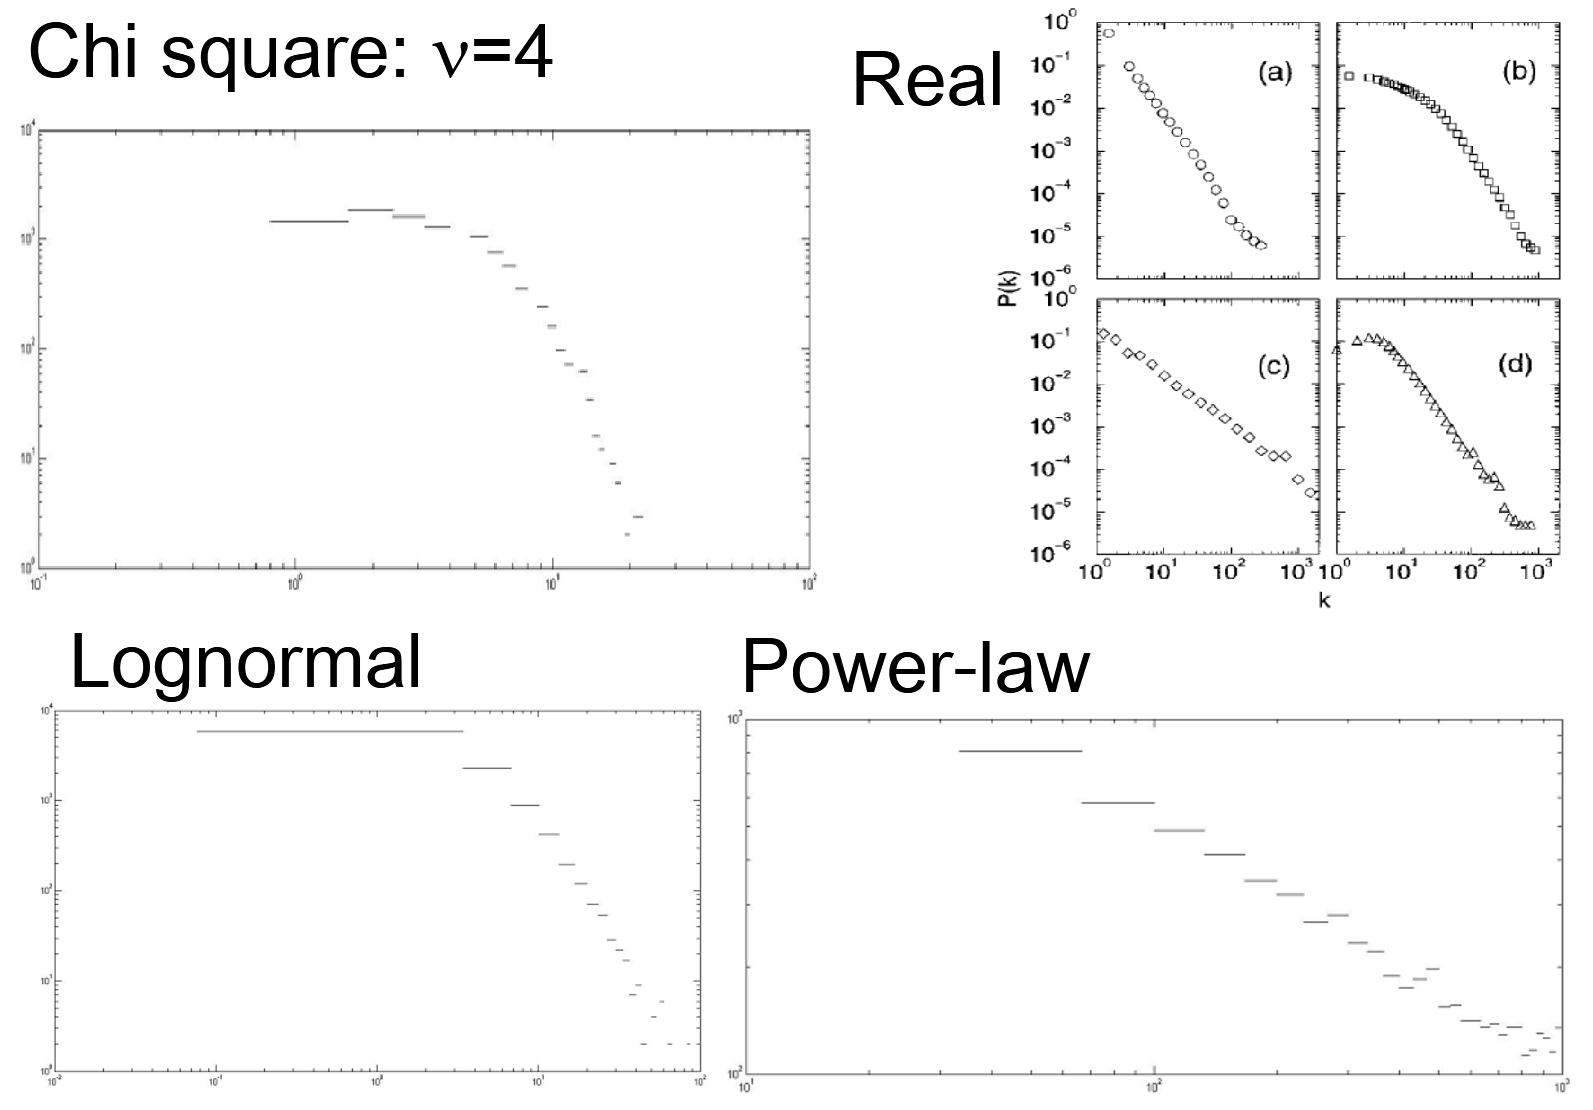
\includegraphics[width=0.8\textwidth]{img/scale_free_real_theory.png}
    \end{minipage}
    \hfill
    \begin{minipage}{0.35\textwidth}
        \caption{Schematic log-log plot comparing comparing theoretical distributions (Chi-square, Lognormal, Power-law) with empirical Real network data, illustrating how visually similar different fat-tailed distributions can appear for small datasets.}
    \end{minipage}
\end{figure}

\textit{Crucial Note:} Why does this distinction matter? Because \textbf{other probability distributions require completely different generative models!} If a real network is actually lognormal, attempting to model its growth using standard B-A preferential attachment is physically and mathematically incorrect.

\subsubsection{Mathematical Forms of Fat-Tailed Distributions}

For reference, here are the formal probability density functions of the most common fat-tailed distributions that often masquerade as power-laws in empirical network analysis:

\begin{itemize}
    \item \textbf{Lognormal:}
          \[
              p(x) = \frac{1}{x\sqrt{2\pi\sigma^2}} e^{-\frac{(\log x - \mu)^2}{2\sigma^2}}
          \]
    \item \textbf{Gamma:}
          \[
              p(x) = \frac{1}{\Gamma(k)\theta^k} x^{k-1} e^{-\frac{x}{\theta}}
          \]
    \item \textbf{Weibull / Stretched Exponential:}
          \[
              p(x) = \frac{k}{\lambda} \left(\frac{x}{\lambda}\right)^{k-1} e^{-\left(\frac{x}{\lambda}\right)^k}
          \]
\end{itemize}

\subsubsection{The B-A Model and the Problem of Non-Locality}

Beyond the exact shape of the degree distribution, there is a fundamental theoretical flaw in the strict Barabási-Albert model. As we know, the degree distribution \( p(k) \) is not the only salient feature of a network; different generative methods can lead to the exact same \( p(k) \) but yield different topological properties (like clustering or assortativity) that uniquely characterize them.

The most glaring physical unrealistic assumption of the pure B-A model is its \textbf{non-locality}.
The preferential attachment mechanism mathematically dictates that the probability of a new node connecting to node \( i \) is \( \frac{k_i}{\sum_j k_j} \).

To calculate this probability, the new node must somehow know the exact degree of node \( i \), as well as the degrees of \textit{all other nodes} in the entire network simultaneously. This implies \textbf{perfect global information}.

Is it always possible to have this information in real systems? \textbf{In general, it is not.}
When a new person joins a social network, they do not scan the friend counts of all 3 billion users to decide who to follow. When a new website is created, the webmaster does not globally evaluate the in-degree of every single page on the internet. Real networks grow based on \textbf{local information}, random walks, and local searches, making the global non-local requirement of the strict B-A model an abstract mathematical convenience rather than a true physical reality.

\section{The Duplication Model}

\subsection{Topologies of Biological Systems}
When we analyze biological networks, such as the proteome (protein-protein interaction networks), we observe a specific set of topological features that are not fully captured by standard random graphs or pure Barabási-Albert (B-A) scale-free models.

Specifically, these biological systems exhibit:
\begin{itemize}
    \item A degree distribution \( p(k) \) that is broadly \textbf{scale-free but with an exponential cutoff} (yielding a Gamma-like distribution, as older nodes do not grow infinitely).
    \item A significantly \textbf{higher level of clustering} compared to random networks, maintaining strong "small-world" properties (high local modularity alongside short global path lengths).
\end{itemize}
The fundamental question arises: how can we theoretically generate these specific topological features by taking into account the actual, physical "biological" properties of the system?

\subsubsection{The Biological Mechanism: Gene Duplication and Mutation}
In biology, the basic functional mapping is \textbf{Gene \( \rightarrow \) Protein}. During cell division and DNA replication, random errors occur.

One of the most critical macroscopic errors for evolutionary network development is \textbf{Gene Duplication}: a gene is entirely "copied" several times. Immediately after duplication, the new gene produces the exact same protein as the original, meaning it perfectly inherits all the original protein's network interactions (links).

However, over evolutionary time, \textbf{mutations} accumulate inside the duplicated gene. These mutations progressively modify the produced protein's structure. Consequently, its initial set of functional interactions is modified—some original interactions are \textbf{lost}, and completely new functional interactions are \textbf{added}.

\subsubsection{Historical Context: Darwin and Haldane}
The evolutionary power of structural duplication was recognized long before modern network science.

In \textit{On the Origin of Species} (1859), Charles Darwin noted the evolutionary flexibility of redundant structures:
\begin{quote}
    \textit{"We have formerly seen that parts many times repeated are eminently liable to vary in number and structure; consequently it is quite probable that natural selection, during the long-continued course of modification, should have seized on a certain number of the primordially similar elements, many times repeated, and have adapted them to the most diverse purposes."}
\end{quote}

Later, in 1932, J.B.S. Haldane formalized this genetically. He suggested that gene duplication events are highly favorable because they produce "spare" genes. These redundant copies can be freely altered by mutations to develop new functions \textit{without} causing a fatal disadvantage to the organism (since the original gene is still there performing the essential baseline function). Furthermore, organisms with multiple copies of critical genes are statistically less prone to harmful, function-destroying mutations.

\subsection{The Duplication Model for Directed Networks}
To translate this biological reality into a mathematical network generative model, we define the \textbf{Duplication Model} for a directed network.

At each time step, the network grows according to the following algorithmic rules:
\begin{enumerate}
    \item \textbf{Duplication:} A random target node (representing a gene) with \( m \) links is selected and completely \textbf{duplicated}. A new node is added to the network, and it initially copies all \( m \) links of the target node.
    \item \textbf{Rewiring (Mutation):} For each of the duplicated outgoing links, there is a probability \( P = \alpha \) that the link is \textbf{rewired} to point to a completely different, randomly chosen node in the network (representing the gain of a new functional interaction due to mutation).
    \item \textbf{Maintenance (Conservation):} Conversely, there is a probability \( P = 1 - \alpha \) that the duplicated outgoing link is \textbf{maintained}, continuing to point to the exact same target as the original gene's link.
\end{enumerate}

By applying these simple, biologically motivated rules of copy-and-mutate, the network naturally develops highly clustered communities (because duplicates share neighbors) while still producing hubs. The mathematical challenge then becomes: under these specific generative rules, \textbf{how does the incoming connectivity of the nodes vary asymptotically?}

\subsection{Mathematical Formulation of the Duplication Model}

To mathematically understand how the duplication-mutation mechanism shapes the network, we can analyze the growth of a generic node's incoming connectivity \( k_{in} \) using a continuous approximation, similarly to what we did for the Barabási-Albert model.

In this directed network model, when a new node is added (representing a duplicated gene), an existing node in the network:
\begin{enumerate}
    \item Receives \( m \) \textbf{new links} directly from the newly added node with a probability \( \alpha \).
    \item Receives \textbf{"old" links} (proportional to its existing degree, as its incoming neighbors are duplicated) with a probability \( 1 - \alpha \).
\end{enumerate}

\subsubsection{Continuous Approximation and the Differential Equation}
Assuming the total number of nodes \( N \) grows linearly with time (\( N \simeq t \)), we can write the differential equation for the time evolution of the incoming degree \( k_{in,i}(t) \) of a specific node \( i \):
\[
    \frac{\partial k_{in,i}(t)}{\partial t} = (1 - \alpha)\frac{k_{in,i}(t)}{N} + m\frac{\alpha}{N}
\]
Substituting \( N \simeq t \), we get:
\[
    \frac{d k_i}{dt} = \frac{[(1 - \alpha)k_i + m\alpha]}{t}
\]
To solve this separable differential equation, we introduce a change of variable: let \( k' = (1 - \alpha)k_i + m\alpha \), which implies \( dk' = (1 - \alpha)dk_i \). The equation rewrites as:
\[
    \frac{dt}{t} = \frac{dk'}{(1 - \alpha)k'}
\]
Integrating both sides from the node's birth time \( t_i \) to current time \( t \):
\[
    \ln\left(\frac{t}{t_i}\right) = \ln\left( (k')^{\frac{1}{1 - \alpha}} \right)
\]
By exponentiating and isolating the birth time \( t_i \), we obtain the relation between a node's age and its transformed degree:
\[
    t_i = t \cdot (k')^{-\frac{1}{1 - \alpha}}
\]

\subsubsection{Degree Distribution: A Shifted Power-Law}
Assuming linear growth of the network (where the birth times \( t_i \) are uniformly distributed, as in the standard B-A model), we can calculate the Cumulative Density Function (cdf). The probability that a node has a degree smaller than \( k' \) is proportional to the probability that its birth time \( t_i \) is greater than the corresponding threshold:
\[
    cdf: P(k'_i < k') = P\left( t_i > t \cdot (k')^{-\frac{1}{1 - \alpha}} \right) \propto (k')^{-\frac{1}{1 - \alpha}}
\]
Substituting \( k' \) back with our original variables, the cdf takes the form:
\[
    cdf \propto [(1 - \alpha)k + m\alpha]^{-\frac{1}{1 - \alpha}}
\]
Finally, to find the Probability Density Function (pdf), we take the derivative of the cdf with respect to \( k \):
\[
    pdf: \frac{d(cdf)}{dk} = p(k_{in}) \propto \left[ k_{in} + \frac{m\alpha}{1 - \alpha} \right]^{-\frac{2 - \alpha}{1 - \alpha}}
\]

\textbf{Key Takeaway:} The resulting degree distribution is a \textbf{shifted power-law} of the form \( (x + a)^b \).
The mathematical structure is strictly analogous to the B-A model with \textbf{initial attractiveness} (where the probability was proportional to \( k + A \)). However, here the interpretation is entirely different: the shift and the exponent are not arbitrary constants, but emerge directly from the biological mutation probability \( \alpha \). This model naturally allows for the \textbf{tuning of the scale-free polynomial exponent} simply by varying the mutation rate.

\subsection{Implicit Preferential Attachment}
One of the most elegant features of the duplication model is that it generates a scale-free topology \textbf{without an explicit preferential attachment rule}. We do not need a mechanism where nodes consciously "seek out" the most connected hubs.

Instead, the preferential attachment is \textbf{implicit}. By uniformly choosing a gene to be duplicated at random, the genes that have already been successfully duplicated many times in the past (forming large functional families) are statistically more likely to have one of their members chosen again.
Mathematically, the probability of duplicating a specific type of node is:
\[
    p_{DUPL}(i, t) = \frac{\text{NODE}_i}{\sum \text{NODE}(t)}
\]
Because of this statistical redundancy, the probability of getting new links naturally ends up being proportional to the node's incoming degree, perfectly mimicking the "rich get richer" effect through pure blind duplication.

\subsection{The Chinese Restaurant Process (CRP)}
This generative process for the evolution of node degree is heavily analogous to a famous concept in probability theory known as the \textbf{Chinese Restaurant Process (CRP)}.

Imagine a restaurant with an infinite number of tables, each capable of seating an infinite number of people. When a new customer enters:
\begin{itemize}
    \item They choose to sit at an \textbf{already occupied table} with a probability proportional to the number of customers already seated there (representing the duplication of an existing link, probability \( \alpha \)).
    \item Alternatively, they choose to sit at a \textbf{completely new, unoccupied table} with a constant probability (representing a mutation leading to a novel interaction, probability \( 1 - \alpha \)).
\end{itemize}
This dynamic leads to the exact same heavy-tailed distribution of customers at tables as we see with links connecting to biological nodes.

\subsection{Duplication Model and the World Wide Web}
While primarily formulated to explain biological evolution, the duplication model is universal enough to describe human technological systems.

A strikingly similar mechanism can be imagined for the creation of \textbf{new websites on the WWW}. When people create a new website (e.g., a blog, a course page, a repository), they rarely build their link structure from absolute scratch. Instead, they often "duplicate" the structure of an existing, similar website—copying its hyperlinks to other external resources—and then apply personal modifications (adding new links or deleting old ones). This simple copy-and-edit human behavior naturally leads to the strongly clustered, scale-free structure of the Internet.